%
% Template for a Thesis
%
\documentclass[a4paper,12pt,oneside]{book}
\linespread{1.2}
\usepackage[left=3.5cm, right=2.5cm, top=3.5cm, bottom=3.5cm]{geometry}
%\usepackage[latin1]{inputenc}
\usepackage[english]{babel}
\usepackage{amsfonts,amsmath,amssymb,amsthm,color}
\usepackage{graphicx}
\usepackage{float}
\usepackage{emptypage}
\usepackage{titlesec}
\usepackage{algorithm,algcompatible}
\usepackage{tabularx}
\usepackage[utf8]{inputenc}
\usepackage{subcaption}
\usepackage[hidelinks]{hyperref}
\usepackage[font=small,labelfont=bf]{caption} % caption belle alle figure
\usepackage{algorithm}
\usepackage{algpseudocode}
\usepackage{booktabs} % Per linee orizzontali migliori
\setcounter{tocdepth}{5}

\usepackage[
backend=bibtex,
style=ieee,
sorting=none
]{biblatex}

\addbibresource{thesis_bib.bib} % put your bibliography here

\newtheorem{theorem}{Theorem}


\raggedbottom

\graphicspath{{figs/}}

\begin{document}
	


%%%%%% First Page %%%

\pagestyle{myheadings}


\thispagestyle{empty}  
                                               
\begin{center}                                                            
    \vspace{2mm}
    {\large ALMA MATER STUDIORUM -- UNIVERSIT\`A DI BOLOGNA} \\  
                         
      \vspace{2mm}
\end{center}
\begin{center}

\end{center}
\begin{center}
      \vspace{5mm}
      {\large \uppercase{School of Engineering}} \\
        \vspace{5mm}
       {\large Department of\\
       Electrical, Electronic and Information Engineering\\
   		``Guglielmo Marconi''}\\
   		{\large DEI}\\
        \vspace{5mm}
      {\Large \bf Master's Degree in Automation Engineering}\\
      \vspace{5mm}
      { \textbf{Master Thesis}\\ in\\ \textit{Optimal Control}}\\
      \vspace{5mm}
      {\LARGE\bf Control of an autonomous aerodynamic airshield for training Olympic 100m sprint athletes} \\                
      \vspace{15mm}
      
      % table??
		\begin{tabularx}{\textwidth} { 
				>{\raggedright\arraybackslash}X 
				>{\raggedleft\arraybackslash}X }
				{\large Candidate:}& 	{\large Supervisor:} \\[3mm]
				{\large \itshape  Giulia Cutini} & {\large \itshape Prof. Giuseppe Notarstefano} \\[3mm]
				& {\large Co-supervisor:} \\[3mm] 
				& {\large \itshape Prof. Melanie Zeilinger} \\
                & {\large \itshape Dr. Andrea Carron} \\
                & {\large \itshape Ing. Lorenzo Sforni} \\
		\end{tabularx}
      \vfill
      {\large Academic Year \\ \itshape 2022--2023} \\
      \vspace{5mm}
      {\large Session \\ \itshape IV}
\end{center}


\vfill

\newpage
\thispagestyle{empty}



%%%%%%FRONTESPIZIO%%%%%%

%%%%%% ABSTRACT %%%%%%%%%%


\chapter*{Abstract}
% \addcontentsline{toc}{chapter}{Abstract}


%%%%%% INDEX %%%%%%%%%%

\tableofcontents
\thispagestyle{empty}

%%%%%%% BODY %%%%%%%%%

\chapter*{Introduction}
\addcontentsline{toc}{chapter}{Introduction}
\markboth{}{INTRODUCTION}
	
\section*{Motivations}
\addcontentsline{toc}{section}{Motivations}

In contemporary times, the integration of advanced technologies has become an integral facet of sport, ushering in a new era of innovation and performance enhancement \cite{Technology_athletics}. 
In sports characterized by high-speed competition, where victories are often determined by mere thousandths of a second, the advancements in technology have revolutionized performance across various disciplines. 
\bigskip

The development of streamlined swimsuits with advanced materials reduces drag and enhances buoyancy, leading to faster times in competitive swimming events.
Ski manufacturers utilize materials like carbon fiber and titanium in ski construction, resulting in lighter yet more stable skis that offer better control and responsiveness on the slopes.
The incorporation of carbon fiber also into athletic footwear has not only reduced weight but also enhanced energy return and propulsion, while concurrently mitigating the risk of injury.
\bigskip

The exploitation of technology for improving performances is not only used for competitions but also during the training phase. 
In the track and field context, several training techniques have been used for the enhancement of running speed. 
Among several possibilities overspeed training involves performing exercises or movements at a velocity higher than what the athlete can achieve through voluntary effort. 
Many methods for experience supramaximal velocities during trainings have been proposed: the usage of assistance mechanisms such as bungee cords or sleds is analized in \cite{Elastic_cord} and is found to be potentially dangerous for sprinters, requiring body contact with an external tool.
Performing sprints on a downward slope allows to accelerate beyond typical maximal speed due to assistance provided to gravity force \cite{Hill_slope}.
\bigskip

In the context of gaining a training edge in sprint events the concept of aerodynamic drag resistance assumes a paramount importance. 
Accordingly sprinters meticulously refine their body position, posture, and apparel to minimize aerodynamic drag. 
For this reason CONI (Italian National Olympic Committee) Institute of Sports Science presented in 2021 an aerodynamic shield to drastically reduce the resistance to forward movement  during sprinters' training \cite{Coni_article}. 
This shield allows athletes to run in the slipstream behind a car pulling the shield, experiencing speeds higher than those of the competition but with the same power output. 
\bigskip

Advancement in automated driving technology has created opportunities for many fields and autonomous vehicles (AVs) have become increasingly prevalent. 
Given their versatility and potential to enhance efficiency and convenience, it's natural to consider their application in the realm of sports. 
Similarly to the user-cooperative robots, designed to stay in direct contact with humans and assist them in several situations, an autonomous vehicle has been designed for driving the aerodynamic airshield. 
Furthermore, intelligent control algorithms have shown huge advantages in autonomous system control, taking into account factors such as control error, bound constraints on system actuators, disturbance rejection and safety guarantees. Additionally, control algorithms can be designed to continuously monitor and analyze data from various sensors in real-time, enabling them to detect and respond to potential hazards or deviations from safety protocols more effectively than human operators.
\bigskip

This thesis is the result of an abroad internship in ETH (Eidgen\"ossische Technische Hochschule) Z\"urich, with the purpose of designing a proper controller to regulate an autonomous go-kart pulling a plexiglass airshield, according to the runner behaviour.

		
\section*{Literature}
\addcontentsline{toc}{section}{Literature}
Numerous control techniques have been used in the last decades to enhance the efficiency of AVs in several different contexts.
Longitudinal control of automated vehicles has received attention since the 1960s, and possibly even earlier.
\cite{Review_AVCS} gives an historical review of advanced vehicle control systems and longitudinal control of automated vehicles. 
The control of vehicle acceleration to achieve a desired speed profile, essential keypoint of longitudinal control, is the main purpose of this thesis.

\bigskip
The initial and simplest approach adopted to control the go-kart, which must maintain a constant reference position and velocity, relative to the runner behind it, involved a cascade of two Proportional-Integral-Derivative (PID) controllers.
The first PID controller regulates the kart's position and generates a reference velocity for the second controller, a velocity PID.

While PID controllers are widely used in industrial applications due to their straightforward implementation, they were not the optimal choice for this application.
The main challenges of this control scheme includes difficulty in parameter tuning, in handling multi-variable processing and in addressing the initial phase of motion, where the runner's acceleration exceeds the kart's maximum capability, together with the impossibility of predicting the future motion of vehicle. 

\bigskip
The task for which the controller has to be designed is quite similar to adaptive cruise control (ACC), where the goal is to maintain a safe distance from the vehicle ahead while also adjusting the speed to match changing traffic conditions.
Similarly, in this scenario, the controller aims to ensure that the go-kart maintains a consistent position and velocity relative to the runner, analogous to how an adaptive cruise control adjusts the speed of a vehicle to maintain a safe following distance.

\bigskip
Thanks to the capability of optimal controllers to cover multiple objectives and to predict future vehicle behaviour, Linear Quadratic Regulator (LQR) and Model Predictive Control (MPC) have been widely used for vehicle control in interacting contexts.
In \cite{LQR_acc} distance and relative velocity between preceding and controlled vehicles are used as states to design an LQR controller that gives acceleration of the controlled vehicle as input, in such a way to minimize a proper cost function.
Model Predictive Control is also largely used thanks to its capability of controlling a multi-variable process while satisfying a set of state and input constraints. According to \cite{MPC_basics} the essential elements of this controller are a prediction model that allows future predictions, the definition of an objective function reflecting the desired system behaviour, and constraints on both state and input. In the framework of MPC for adaptive cruise control, in \cite{MPC_acc_first} the same state and input variables than in \cite{LQR_acc} are used but constraints can be also incorporated. Differently, in \cite{MPC_acc_second} the controlled vehicle velocity is added as a third state and the acceleration of the preceding vehicle is included in the prediction model, regarded as an unknown external disturbance.

\bigskip
The MPC approach is strongly model-based in the sense that uses a model of the system to produce a prediction of system behaviour. The presence of uncertainties on this model may lead to unsatisfying results of the control task. 
For this reason \cite{Offset-free_compare, Linear_offset-free} show offset-free MPC formulations able to achieve output tracking of reference signals despite the presence of Model-Plant Mismatch (MPM).
For this purpose an augmented predictive model added with an artificial constant disturbance that represents modeling uncertainties, is used. 
To estimate both state ad disturbance from output measurements a disturbance observer must be properly designed and added in conjunction with feedback control law.
Accordingly to \cite{Disturbance_observer} by appropriately including a disturbance estimate in a control law, MPM effects can be approximately removed in steady-state and offset-free tracking of constant references can be achieved.


	
\section*{Contributions}
\addcontentsline{toc}{section}{Contributions}
The main contribution of this thesis lies in the analysis and implementation of linear controllers for a pioneering autonomous driving go-kart, which is utilized for towing the airshield during the training of Olympic athletes participating in the 100m event.
Specifically, the thesis proposes and compares two different control schemes in terms of performances and control architecture.

\bigskip
Initially, a non linear model that accurately captures the dynamics of the kart with the airshield attached is identified. 
Later a good linear approximation is found and used as basis for the design of the predictive controllers.
The first step in control development involves the design of a Linear Quadratic Regulator (LQR) with a gain scheduling approach, where Q and R parameters vary depending on the motion phase. This gain scheduling approach addresses the challenges associated with the different maximum accelerations of the kart and of the runner in the first phase of the motion.
Subsequently, a Model Predictive Control (MPC) is designed with the purpose of incorporate information on the runner future expected behaviour into the linear prediction model.
Furthermore, since MPC is highly model based a disturbance observer and Offset-free MPC has been implemented with the purpose of increasing the accuracy of the predictive model and to obtain a zero-offset in tracking peace-wise affine (PWA) reference trajectories.

\bigskip
The depicted workflow highlights how the control scheme architecture has been simplified starting from the two control loops governing the cascade of PID controllers. The gain scheduling LQR, which switches between two different control gains depending on the motion phase, just makes use of two different regulators. Ultimately, this thesis culminates in a single MPC controller capable of governing the system under all possible operating conditions, integrating information about the future evolution of the runner's velocity profile into the prediction model to further enhance tracking performance.

\bigskip
Both controllers have been developed and tested in simulation using Python and on the real system using ROS2.

\section*{Organization}
This section provides to the reader a guide to the organization of the thesis. 

In Chapter 1 a theoretical background and an overview of the fundamental methodologies used in the control design are presented. 

Chapter 2 is focused on discussing the problem set-up, the formulation of the optimal control techniques developed to accomplish the desired task, in particular the Linear Quadratic Regulator (LQR) and the Model Predictive Control (MPC), in the specific context of this application.

Chapter 3 gives a description of the system mechanical structure, hardware and sensors. Then it shows the numerical results of the controllers application obtained both in Python simulation and on the real hardware. A comparison of the performance in different scenarios is also presented.
This demonstrate the effectiveness of the proposed methodologies.

\chapter{Theoretical Background}
%\addcontentsline{toc}{chapter}{Theoretical Background}
\markboth{}{THEORETICAL BACKGROUND}
%\label{chapter:Theoretical_Background}
In this chapter the aim is to provide the necessary theoretical background for thoroughly understand the design process and the main peculiarities and limitations of the designed controllers: the Linear Quadratic Regulator (LQR) and the Model Predictive Control (MPC).

Optimal control theory provides a mathematical framework for addressing control theory problems by optimizing control laws with respect to given cost functions. The primary goal is to find a control strategy for a given system while penalizing deviations of the system's states or inputs from desired values.
This approach enables achieving optimal system regulation, maximizing control effectiveness, and minimizing the adverse effects of variations in operating conditions or external disturbances.

Such theoretical analysis is essential for fully comprehending the features and performance of the LQR and MPC controllers discussed in Chapter 2 within the specific context of the considered application.

\section{Linear Quadratic Regulator}
In 1960, Kalman pioneered with the field of linear-quadratic feedback control, laying the groundwork for what later became known as the Linear Quadratic Regulator (LQR) \cite{kalman_contributions} in the continuous-time context. 
The LQR is a feedback control algorithm designed to stabilize and optimize the performance in case where the dynamical system can be described by linear equations and the cost function is quadratic in terms of the states and inputs. 

\bigskip
Assuming the process to be controlled to have a good discrete-time LTI description like the following state-space form:
\begin{equation} 
\begin{aligned}
    x^+ &= A x + B u \\
    y &= C x
\end{aligned}
\label{eq:Linear_model}
\end{equation}

where $x \in \mathbb{R}^n$ is the actual system state, $u \in \mathbb{R}^m$ is the system input and $y \in \mathbb{R}^p$ is the measured output, all considered at a certain discrete time instant $t$. 
The state at the subsequent time instant $t+1$ is referred to as $x^+$.

$A \in \mathbb{R}^{n\times n}$ and $B\in \mathbb{R}^{n\times m}$ are the state transition and input distribution matrices, respectively.
In the context of this thesis is possible to assume the full state information available, thus $C \in \mathbb{R}^{p\times n}$ is the identity. 

The primary goal of the control task is to achieve optimal regulation of the system's state towards the origin. 
The notion of optimality, in this context, is framed within a quadratic objective function.
The LQR problem, therefore, can be viewed as a multi-objective optimization task, where the goal is to simultaneously minimize competing objectives.
For example, minimizing the deviation of the system's states from desired values may require higher control effort, and vice versa.
In the context of multi-objective optimization, the challenge lies in finding a balance between these conflicting objectives and this always involves making trade-offs to achieve a satisfactory solution.

\bigskip
The Infinite Horizon Linear Quadratic Regulator problem is defined as follows:
find the optimal control input $u_t, \, \forall t \in [0, \infty)$ that makes the following quadratic criteria as small as possible
\begin{equation}
    J(\boldsymbol{u}, \boldsymbol{u})  = \sum_{t=0} ^{+\infty} x_t^T Q x_t + u_t ^T R u_t
\label{Quadratic_cost_funct}
\end{equation}
where $Q \in \mathbb{R}^{n \times n}$ and $R \in \mathbb{R}^{m \times m}$ are symmetric positive-definite weight matrices.

The vector $\boldsymbol{u}$ contains the input trajectory, i.e. $\boldsymbol{u} = \{u_0, u_1, \dots\}$ and $\boldsymbol{x}$ is the one containing the state trajectory, i.e $\boldsymbol{x} = \{x_1, x_2, \dots\}$.
The cost function in \ref{Quadratic_cost_funct} can be seen as the mathematical formulation of the trade-off between the two objectives to be minimized.
Specifically the term $x_t^T Q x_t$ penalizes deviations of the system's states from desired values, while $u_t^T R u_t$ penalizes excessive control effort.
The weights of the $Q$ and $R$, typically chosen as diagonal matrices, can be adjusted to find solutions that strike an appropriate balance between minimizing state deviations and control effort.


\bigskip
Assuming the pair $(A,B)$ to be controllable and the pair $(A,C)$ with $Q = C^T C$ to be observable, holds:
\begin{itemize}
    \item there exists a unique positive definite $P_\infty$ solution of the following equation called Algebraic Riccati Equation (ARE)
    \begin{equation}
        P_\infty = Q + A^T P_\infty A - A^T P_\infty B (R + B^T P_\infty B)^{-1} B^T P_\infty A.
    \end{equation}
    \item exploiting the first-order necessary and sufficient conditions for optimality, the optimal control law is a closed form solution, feedback of the state
    \begin{equation}
        u_t^* = K x_t^*
    \end{equation}
    with
    \begin{equation}
        K = -( B^T P_\infty B + R)^{-1}(B^T P_\infty A)
    \label{eq:Regulator_LQR}
    \end{equation}
    and it is able to asymptotically stabilize the system.
\end{itemize}

The pair $(x_t^*, u_t^*)$ is the optimal state and input at discrete time instant $t$.

\bigskip
Despite the fact that one of the main applications of LQ optimal control is regulation, this strategy can be used to track a desired system behaviour as closely as possible, in the framework of Linear Quadratic Tracking (LQT).
To incorporate the desired behaviour to be tracked in the objective, the problem can be written as:
\begin{equation}
\begin{aligned}
	\min_{\substack{\boldsymbol{x}, \boldsymbol{u}}}\quad J &= \sum_{t=0}^{+\infty}  (x_t - x_{t,\text{des}})^T Q (x_t - x_{t,\text{des}}) + u_t^T R u_t  \\
	\text{subj. to} & \quad x_{t+1}  = A x_t + B u_t \hspace{2cm} t = 0, 1 \ldots. \\
    & \quad x_0 = x_{\text{init}}
\end{aligned}
\label{eq:LQR}
\end{equation}

where $x_{\text{des}}$ is the reference signal we want our system's states to track over time.

Cost function quantifies the controlled system's performance, defined as a weighted sum of the deviations of the system's states from desired values and control effort.

In the context of tracking piece-wise affine desired state behaviour the optimal feedback control law is modified in the following way:
\begin{equation}
    u_t^* = K (x_t - x_{t,\text{des}})
\label{Closed-loop_control_law}
\end{equation}
where the term $x_t - x_{t,\text{des}}$ is the tracking error at time $t$.

The effectiveness of LQR lies in its ability to leverage the full state information of the system, enabling precise and efficient control.


\section{Linear Model Predictive Control}
Model Predictive Control (MPC) is a modern control strategy renowned for its capacity to provide optimized responses while accounting for state and input constraints, such as saturation limits.
These constraints can be explicitly integrated into the control design, enhancing the robustness and performance of the system. 
The origin of MPC trace back to the mid-seventies to mid-eighties, initially emerging in industrial applications. 
However, it was not until the nineties that MPC theory underwent significant advancements, leading to its widespread adoption and refinement.

\bigskip
MPC relies on the provided dynamic model to predict the behaviour of the system and determine the optimal control action based on the chosen performance criteria. 
A key aspect of MPC design is selecting a suitable model, one that adequately describes the system's dynamics while maintaining simplicity to ensure tractability and real-time solvability of the optimization problem.

\bigskip
The description of the linear discrete-time system prediction model is the same shown in \ref{eq:Linear_model}.

For what regards the states and inputs constraints they can be expressed as follows
\begin{align}
    x_t & \in \mathcal{X} \\
    u_t & \in \mathcal{U}
\end{align}
the state set $\mathcal{X}$ is closed and the input set $\mathcal{U}$ is compact and non-empty. Usually the sets are described with linear inequalities and both sets are convex and contain the origin.

\bigskip
Similarly to the LQR case, Model Predictive Control aims to minimize a cost function by defining positive definite matrices $Q$ and $R$. The goal is to find the optimal control input that minimizes a cost function that takes the following form:
\begin{equation}
    J(x_t, \boldsymbol{u}, t) = \sum_{i=t} ^{+ \infty} x_{i|t}^T \, Q \, x_{i|t} + u_{i|t}^T \, R \, u_{i|t}
\end{equation}

In this formulation $x_{i|t}$ represents the predicted state a time $i$, given the actual state $x_{t|t}$. 
Similarly, $u_{i|t}$ is the predicted control sequence at current time $t$ found considering the entire future predicted trajectory for the system.

The aforementioned formulation represents the infinite horizon MPC problem, that in many practical cases results challenging to be implemented or requires highly demanding computations.
For this reason usually MPC formulations optimize only on a finite horizon $N$, thus the problem of tracking $x_{\text{des}}$ with the system's states becomes:

\begin{equation}
\begin{alignedat}{2}
	\min_{\substack{\boldsymbol{x}, \boldsymbol{u}}}\quad J &= \sum_{i=t}^{t+N-1} (x_{i|t} - x_{t,\text{des}}) ^T \, Q \, (x_{i|t} - x_{t,\text{des}}) +  u_{i|t}^T \, R \, u_{i|t} &&   \\
	\text{subj. to} & \quad x_{i+1|t}  = A x_{i|t} + B u_{i|t}   \hspace{2cm} t = 0, 1 \ldots. &&  \\
     &\quad x_{i|t} \in \mathcal{X} && \\
    &\quad u_{i|t} \in \mathcal{U} && \\
    &\quad x_{t|t} = x_{\text{meas}} && 
\end{alignedat}
\label{MPC1}
\end{equation}

\begin{figure}
	\centering
	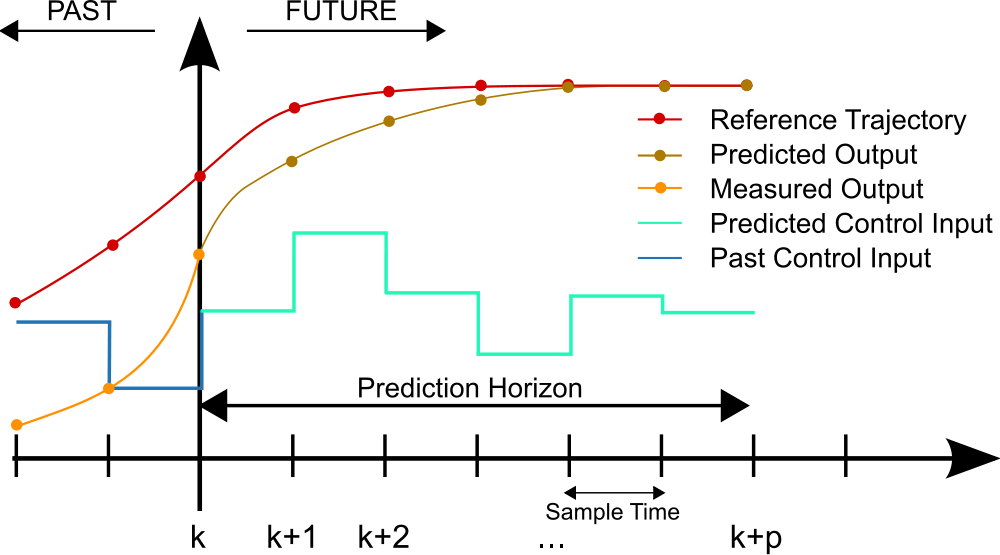
\includegraphics[width=0.66\textwidth]{MPC.png}
	\caption{Model Predictive Control receiding horizon scheme}
	\label{image:mpc}
\end{figure}

\bigskip
The control law is applied based on the receding horizon principle, which is a key feature of MPC.
This principle dictates that at each time instance $t$, an open-loop optimal control problem is solved using the current state of the plant $x_{\text{meas}}$ as the initial state, in order to obtain the control action. 
All predicted states and inputs within a prediction horizon $N$ are optimized to find an optimal input sequence.
However, only the first input of the optimal control sequence generated by the optimization is injected into the plant. 
This input is used to control the system over the next time step.
This procedure is repeated, as illustrated in figure \ref{image:mpc}, at each time instance and by continuously updating the control action based on the most recent information, MPC ensures that the control strategy adapts to changes in the system dynamics and external conditions over time.




\section{Offset-free tracking MPC and disturbance observer}
Even if MPC is able to react to small unmodeled dynamics effects through the receding-horizon fashion, it is not able to consider them inside the predictions, thus to optimize upon them.
MPC solves at each time an optimal control problem using the nominal model of the controlled process and, only when the actual plant behaviour closely matches the nominal model, the feedback control scheme can be guaranteed to stabilize the system, and achieve precise tracking of desired setpoints without any offset.

Offset-free Model Predictive Control represents and advanced control strategy designed to address this limitation. It aims to achieve zero steady-state tracking errors in the controlled system, even in presence of disturbances or model uncertainties that cause model-plant mismatch.
For instance, in the context of regulating nonlinear systems using a linear predictive control framework, offset-free MPC seeks to regulate the system to its desired setpoint without steady-state error, ensuring precise and accurate control performance.

\bigskip
Consider a discrete-time, time-invariant system describing the plant:
\begin{equation}
\begin{aligned}
    x_p^+ &= f_p (x_p, u) \\
    y_p^+ &= h_p (x_p) 
\end{aligned}
\label{Plant1}
\end{equation}
where $x_p \in \mathbb{R}^n$, $u \in \mathbb{R}^m$ and $y_p \in \mathbb{R}^p$ are the state, input and plant measured output respectively. 

The aim of the offset-free model predictive controller is to have $y_p$ tracking a certain reference signal $y_{\text{des}} \in \mathbb{R}^p$ that is assumed to asymptotically converge to a constant.

\bigskip
Let $w \in \mathbb{R}^n$ and $v \in \mathbb{R}^p$ be defined as:
\begin{equation}
\begin{aligned}
    w & := f_p (x_p, u_t) - (A x + Bu) \\
    v & := h_p (x_p) - C x
\end{aligned}
\label{Plant_model_mismatch}
\end{equation}
where the $A$, $B$ and $C$ matrices are the ones mentioned in the linear model \ref{eq:Linear_model}. In particular the $w$ term express the model mismatch between the non-linear plant model and the linear predictive model.

\bigskip
The key feature of this control strategy lies in the incorporation of a disturbance model in the prediction model \ref{eq:Linear_model}.
This is used to estimate and predict the model-plant mismatch between \ref{eq:Linear_model} and \ref{Plant1} in steady state, thus the $w$ term. 

\bigskip
Accordingly, an augmented model is used for computing the system's predictions in the offset-free MPC framework. 
It can be, in general, written in the following form:
\begin{equation}
\begin{aligned}
    x_{t+1} &= A x_t + B u_t + B_d d_t \\
    d_{t+1} &= d_t \\
    y_t &= C x_t + C_d d_t
\end{aligned}
\label{Augmented_model}
\end{equation}
where the additional state $d_t \in \mathbb{R}^{n_d}$ is known as disturbance state or simply disturbance and follows an integral dynamics, as proposed by \cite{pannocchia2003disturbance}. 
The maximum dimension of the disturbance state has to be equal to the number of measured outputs, i.e. $n_d \leq p$.
The pair $(B_d, C_d)$ can be seen as the disturbance model.

\bigskip
Assuming observability of the augmented system \ref{Augmented_model}, an estimator that continuously estimates the augmented state $(x,d)$ can be designed.
An example could be a linear disturbance observer, that uses the prediction error between the real plant output and the predicted one, to estimate the augmented state as described by the following dynamical system:
\begin{equation}
    \begin{aligned}
    	\begin{bmatrix}
    	   \hat{x}_{t+1} \\
            \hat{d}_{t+1}
        \end{bmatrix}
        &= 
    	\begin{bmatrix}
    		A & B_d \\
    		0 & I
    	\end{bmatrix}
    	\begin{bmatrix}
    		\hat{x}_t \\
    		\hat{d}_t
    	\end{bmatrix}
        +
    	\begin{bmatrix}
    		B \\
    		0
    	\end{bmatrix}
        u +
        \begin{bmatrix}
            L_x \\
            L_d \\
        \end{bmatrix} 
        ( - y_{p,t} +
        \begin{bmatrix}
            C & C_d 
        \end{bmatrix}
        \begin{bmatrix}
            \hat{x}_t \\
            \hat{d}_t
        \end{bmatrix} ) \\
        & = A_e 
        \begin{bmatrix}
        \hat{x}_t \\
        \hat{d}_t
    	\end{bmatrix}
        + 
        B_e \, u +
        L (
         - y_{p,t} +
        C_e
        \begin{bmatrix}
            \hat{x}_t \\
            \hat{d}_t
        \end{bmatrix} )
    \end{aligned}
\label{eq:Estimator_and_observer}
\end{equation}
where $\hat{x}$ and $\hat{d}$ are the state and disturbance estimates.

\bigskip
Given the current estimates of the augmented state $(\hat{x}_t, \hat{d}_t)$ the MPC classical formulation is modified into an offset-free MPC algorithm as follows:
\begin{equation}
\begin{alignedat}{2}
	\min_{\substack{\boldsymbol{x}, \boldsymbol{u}}}\quad J &= \sum_{i=t}^{t+N-1} (x_{i|t} - \bar{x}_t) ^T \, Q \, (x_{i|t} -  \bar{x}_t) +  (u_{i|t} - \bar{u}_t)^T \, R \, (u_{i|t} - \bar{u}_t) &&  \\
	\text{subj. to} & \quad x_{i+1|t}  = A x_{i|t} + B u_{i|t} + B_d d_{i|t} \hspace{1.5cm} t = 0, 1 \ldots. &&  \\
    & \quad d_{i+1|t}  = d_{i|t} && \\
    &\quad x_{i|t} \in \mathcal{X} &&  \\
    &\quad u_{i|t} \in \mathcal{U} && \\
    &\quad x_{t|t} = \hat{x}_t && \\
    &\quad d_{t|t} = \hat{d}_t && 
\end{alignedat}
\label{MPC:offset-free}
\end{equation}
where $\bar{x}_t$ and $\bar{u}_t$ are solution of the following system:

\begin{equation}
    \begin{bmatrix}
    A-I & B \\
    C & 0
	\end{bmatrix}
 	\begin{bmatrix}
		\bar{x}_t \\
		\bar{u}_t
	\end{bmatrix}
    =
    \begin{bmatrix}
    -B_d \hat{d}_t\\
    y_{\text{des}} - C_d \hat{d}_t
	\end{bmatrix}
\end{equation}

This optimization cancels the estimated disturbances $\hat{d}_t$ and thanks to this action is able to track the given feasible setpoint with the controlled variables.

\subsection{Observer design}
%\addcontentsline{toc}{section}{Observer design}

In this formulation the nominal augmented state $(x,d)$ needs to be estimated at each time instant, given the plant output measurement $y_p$.

The $L_x \in \mathbb{R}^{n \times p}$ and $L_d \in \mathbb{R}^{n \times n_d} $ observer gain matrices in \ref{eq:Estimator_and_observer} has to be designed in such a way the estimator to be stable, while the method doesn't matter for our purposes.

\bigskip
Two possible choices of state estimator could be Luenberger observer or the Kalman filter. 
Specifically in the context of this thesis the Luenberger observer has been used.
The Luenberger observer updates the state prediction computed at time $t-1$ using the current measured plant output $y_p$ at time $t$ as in the following:
\begin{equation}
    \hat{x}_t = A \hat{x}_{t-1} + B u_{t-1} + L (y_{p,t} - \hat{y}_t)
\end{equation}
where $\hat{y}_t := C(A \hat{x}_{t-1} + B u_{t-1})$.
The difference $(y_{p,t} - \hat{y}_t)$ is called estimation error or correction term and $L \in \mathbb{R}^{n \times p}$ is the observer gain.

\bigskip
If the pair $(A_e,C_e)$ in \ref{eq:Estimator_and_observer} is observable, than the eigenvalues of $(A_e+LC_e)$ can be placed arbitrarily in such a way the estimator dynamical system to be stable.
Usually we want the estimator to be faster with respect to the controller, for this reason the desired eigenvalues for $(A_e+LC_e)$, thus the poles of the estimator dynamical systems, are chosen smaller with respect to the ones of the controlled stabilized system.

\chapter{Control design}
%\addcontentsline{toc}{chapter}{Control design}
\markboth{}{CONTROL DESIGN}
\label{chapter:Control_design}
This chapter will provide first of all a description of the plant model and of the linear approximation used to design the predictive controllers. 

Later on a proper description of the design choices and the formulations of both the controllers in the context of the sport application: the Linear Quadratic Regulator (LQR) and the Model Predictive Control (MPC), nominal and with Offset-free version.

\section{Model}
\begin{figure}[h!]
	\centering
	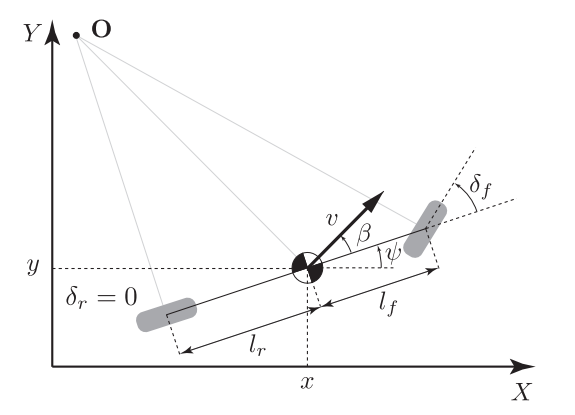
\includegraphics[width=0.7\textwidth]{Bycicle_scheme.png}
\end{figure}
Having a good model plays a central role in the controller design framework.
The non linear model used to describe the kart dynamics is a bicycle model.
2D bicycle model can be seen as a simplified vehicle model that approximates very well the motion of a 4-wheel vehicle in normal driving conditions.

The mathematical equations are the following:
\begin{equation}
\begin{cases}
 	\begin{aligned}
		\dot{x}(t) &= v(t) \cos(\psi(t) + \beta(t)) \\
		\dot{y}(t) &= v(t) \sin(\psi(t) + \beta(t)) \\
		\dot{\psi}(t) &= \frac{v(t)}{l_r} \sin(\beta(t)) \\
		\dot{v}(t) &= \frac{F_x(t)}{m} 
	\end{aligned}
\end{cases}
\label{Plant}
\end{equation}

where $x = [x, y, \psi, v]$ is the state vector where the components are respectively the $x$ and $y$ world frame coordinates, $\psi$ the heading angle with respect to the reference frame, and $v$ the total speed of the vehicle.

The longitudinal force $F_x$ acting on the vehicle is modeled as a single force applied to the center of gravity of the vehicle and is computed as a combination of the drive-train command and the velocity. 
\begin{align}
    F_x (t) &= (C_{m_1} - C_{m_2} v(t)) a(t) - C_f v(t) - C_d v^2(t) - C_{roll} \label{eq:Long_force}\\
    \beta(t) &= \arctan\left(\tan\left(\frac{l_r}{l_f+l_r}\delta_f(t)\right) \right).
\end{align}
The inputs of this system are $u = [a, \delta_f]$ where $a$ is the drive-train acceleration and $\delta_f$ the front steering angle. 
The variable $\beta$ is the slip angle at the center of mass. 

\bigskip
The model has two parameters, $l_f$ and $l_r$, which represent the distances from the centre of mass to the front axle and rear axle, respectively.

The mass $m = 300$ Kg includes both the kart and the trailer weight, while $l_f = l_r = 0.8$ m.
The other parameters of this model have been identified as reported in table \ref{tab:Parameters}.


\bigskip
The identified coefficients represent:
\begin{itemize}
    \item $C_{roll}$ : rolling coefficient modeling the wheel friction on the road surface
    \item $C_d$ : coefficient modeling aerodynamic resistance or drag
    \item $C_f$ : coefficient modeling the dynamic friction resistance
    \item $C_{m1}$ : coefficient associated with the force component due to the driving torque of the vehicle
    \item $C_{m2}$ : coefficient associated with the force component due to both the torque and the velocity
\end{itemize}

\begin{table}[h!]
    \centering
    \begin{tabular}{|c|c|}
        \hline
        $C_{m1}$ & 930 \\
        \hline
        $C_{m2}$ & 0 \\
        \hline
        $C_f$ & 10 \\
        \hline
        $C_d$ & 1.5 \\
        \hline
        $C_{roll}$ & 73 \\
        \hline
    \end{tabular}
    \caption{Identified parameters for bicycle model}
    \label{tab:Parameters}
\end{table}

According to the estimated values the \ref{eq:Long_force} can be rewritten as follows:
\begin{equation}
    F_x(t) = C_{m1} a(t) - C_f v(t) - C_d v^2(t) - Croll
\end{equation}

The physical actuations limits on the input variable $a$ can be expressed as box constraints of the following type:
\begin{equation}
    a_{\text{min}} \leq a_t \leq a_{\text{max}}
\label{Input_limits}
\end{equation}
The coefficients reported in table \ref{tab:Parameters} are identified in such a way to have $a_{min} = 0$ and $a_{max} = 1$ as actuation limits for the motor torque.

\section{Linear approximation of the system dynamics}
The application for which the system is designed is for training Olympics runner in overspeed training. 
Due to the high velocities involved in this kind of training technique, the athlete is interested to execute only distances of about $50/60$ m. 
For this reason it is reasonable to consider only the longitudinal motion of the vehicle along one direction and not taking anymore into account the steering degree of freedom. 
According this assumption the plant model can be simplified as in the following:

\begin{equation}
\begin{cases}
 	\begin{aligned}
		\dot{p}(t) &= v(t) \\
		\dot{v}(t) &= \frac{F_x(t)}{m} = \frac{1}{m} (C_{m1} a(t) - C_f v(t) - C_d v^2(t) - C_{roll} )
	\end{aligned}
\end{cases}
\label{Plant_simplified}
\end{equation}
where $p$ indicates the position of the vehicle along an arbitrarily oriented direction.

\bigskip
It's very easy to notice that a good linear approximation of \ref{Plant_simplified} can be found and used for the controller design. 
The only non linear term is in fact the one related to the drag coefficient in the equation describing the longitudinal force.
Assuming that in the context of this application, the velocities the kart exploits during the motion are quite small, this term will be small as well.

Accordingly, continuous time dynamics equations of the linear approximation model can be obtained by just removing that non linear term:
\begin{equation}
\begin{cases}
 	\begin{aligned}
		\dot{p}(t) &= v(t) \\
		\dot{v}(t) &= \frac{F(t)}{m} = \frac{1}{m} (C_{m1} a(t) - C_f v(t) )
	\end{aligned}
\end{cases}
\label{CT_Linear_dynamics}
\end{equation}

\bigskip
The Forward Euler method is used for discretize the given continuous-time dynamical system:
\begin{equation}
    y_{t+1} = y_t + dt \cdot f(y_t, t) 
\end{equation}
where $f$ is the continuous time function and $dt$ is the discrete-time step size, distance between two consecutive discretization steps.

It is possible to write the following linear discrete-time, time-invariant system:
\begin{equation}
\begin{cases}
	\begin{aligned}
		p_{k,t+1} &= p_{k,t} + dt \, v_{k,t} \\
		v_{k,t+1} &= v_{k,t} + dt \left( \frac{C_{m1}}{m} u_t - \frac{C_f}{m} v_{k,t}  \right)
	\end{aligned}
\end{cases}
\end{equation}

And moving into the state space form it can be rewritten as:
\begin{equation}
    \begin{aligned}
    	x_{k,t+1} = 
    		\begin{bmatrix}
    			p_{k,t+1} \\
    			v_{k,t+1}
    		\end{bmatrix}
    		& =
    		\begin{bmatrix}
    			1 & dt \\
    			0 & 1-dt\frac{C_f}{m}
    		\end{bmatrix}
    		x_{k,t}
    		+
    		\begin{bmatrix}
    			0 \\
    			dt \frac{C_{m1}}{m}
    		\end{bmatrix}
    		u_t \\
    		& = A \, x_{k,t} + B \, u_t
    \end{aligned}
\label{Linear_system}
\end{equation}

where $x_k = [p_k , v_k] ^T$  are the kart state variables expressing respectively the kart position and the kart velocity and $u = a$ is the control input of the system, while $dt$ is the sampling step used for Euler forward integration.

This linear model is the one used as basic for the controllers design in the following.

\newpage
\section{LQR design}
Consider that at each time instant the information about the runner state $x_r =[p_r , v_r] ^T $ is known, where $p_r$ represents the absolute runner position and $v_r$ indicates the absolute runner velocity.

At each time instant $t$ the desired state for the go-kart is given by:
\begin{equation}
    x_{k,\text{des}} =
    \begin{bmatrix}
        p_r + d_{\text{des}} \\
        v_r
    \end{bmatrix}
\end{equation}
where $d_{\text{des}}$ denotes the reference distance between the kart and the runner.
Using this reference, the closed-form control law in \ref{Closed-loop_control_law} is applied to obtain the optimal unconstrained solution $u^*$ , at each time instant.

\bigskip
While MPC explicitly incorporates constraints into the optimization problem, LQR does not provide a direct mechanism for handling constraints.
Constraints in LQR can be indirectly addressed by penalizing their violation in the cost function, but it's still possible to deal with control actions that violate certain physical limits, such as those described in \ref{Input_limits}.
To address this, the unconstrained control actions generated by the LQR controller has been "clipped" as follows:
\begin{equation}
    \Tilde{u}^* = \text{sat}_{[a_{min}, a_{max}]} (u^*)
\end{equation}

The value $\Tilde{u}^*$ can be referred to as the clipped-unconstrained optimal LQR control action.
While clipping allows the controller to handle constraints in a straightforward manner, it can lead to suboptimal performances, as the controller may be forced to operate at the constraint boundaries.
Therefore, alternative approaches such as MPC may be preferred for systems with stringent constraint requirements.

\subsection{Catch-up maneuver}
\begin{figure}
	\centering
	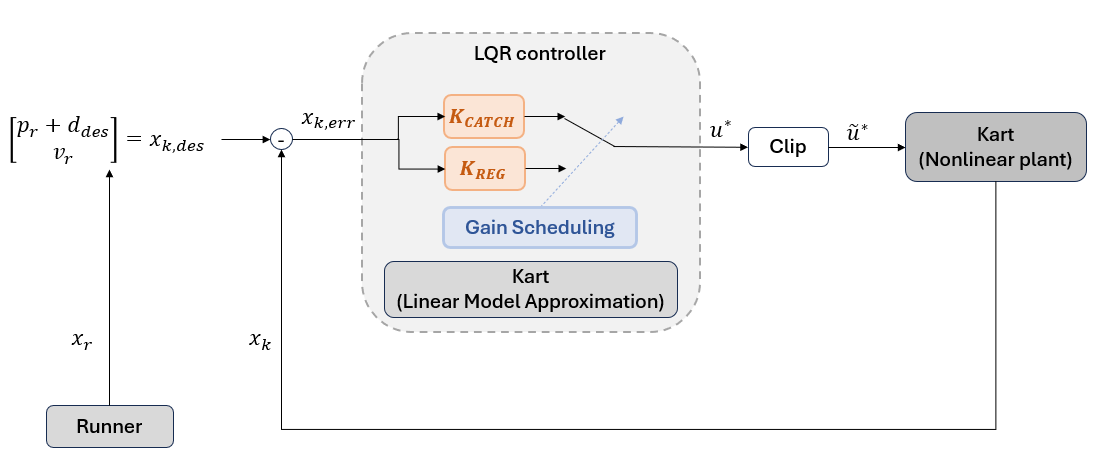
\includegraphics[width=1.0\textwidth]{LQR_sim_scheme.png}
	\caption{Linear Quadratic Regulator control scheme}
	\label{image:LQR_sim_scheme}
\end{figure}

The most challenging phase of the motion occurs in the first few seconds when the runneraccelerates faster than the maximum acceleration the kart can achieve.
This phase is referred to as the 'catch-up maneuver'.
To prevent a potential collision between the airshield and the runner, a safety measure is implemented, requiring the runner to begin the sprint performance from a position several meters farther from the kart, with respect to the steady state desired distance $d_{\text{des}}$.

Hence, the initial condition for the kart state is set to be the following:
\begin{equation}
    x_{k,\text{init}} =
    \begin{bmatrix}
        d_{\text{des}} + \bar{d} \\
        0
    \end{bmatrix}
\end{equation}
where $\bar{d}$ is a parameter that depends on how fast the runner is going to accelerate during his performance. 
 
\bigskip
From the control architecture point of view a gain scheduling approach has been introduced in the control scheme.
During the catch-up phase, the control action is governed by the controller gain $K_{\text{catch}}$ computed using the following weights: 
\begin{equation}
    Q_{\text{catch}} =
    \begin{bmatrix}
        40 & 0 \\
        0 & 1000
    \end{bmatrix},
    \quad
    R_{\text{catch}} = [2]
\end{equation}

As clearly understandable from the weights, during the catch-up maneuver, the primary objective is to match the go-kart velocity with  that of the runner.
Once this alignement is achieved, typically at an 80\% match, the controller switches to $K_{\text{reg}}$ which assigns nearly equal importance to distance and velocity mismatch.
\begin{equation}
    Q_{\text{reg}} =
    \begin{bmatrix}
        1000 & 0 \\
        0 & 4000
    \end{bmatrix},
    \quad
    R_{\text{reg}} = [0.002]
\end{equation}

The overall control scheme is the one shown in \ref{image:LQR_sim_scheme}, while algorithm \ref{alg:LQR_sim_implementation} outlines the steps followed by the LQR algorithm while controlling the system.
\begin{algorithm}
\begin{algorithmic}[1]
	\State catched = false;
	\State Set initial runner position with a proper distance $\bar{d}$ from kart;
	\For{$t=0,1,2,...$};
		\State Take kart state information $x_{k,t} = [p_{k,t}, v_{k,t}]^T$;
		\State Take runner state information $x_{r,t} = [p_{r,t}, v_{r,t}]^T$;
		\State Compute corresponding desired state for kart $x_{k,t,des} = [p_{r,t} + d_{\text{des}}, v_{r,t}]^T$;
		\If{$v_{k,t} \geq 0.8 v_{r,t}$ \textbf{and} catched = false}
			\State catched = true;
		\EndIf
		\If{catched = false}
			\State $u^* = - K_{\text{catch}} (x_{k,t} - x_{k,t,des}) $;
		\Else 
			\State $u^* = - K_{\text{reg}} (x_{k,t} - x_{k,t,des}) $;
		\EndIf
		\State Clip input according to limit saturation limits $\tilde{u}^* = \text{sat}_{[a_{\min}, a_{\max}]} (u^*)$;
		\State Inject $\tilde{u}^*$ in the plant;
	\EndFor
\caption{LQR implementation}
\label{alg:LQR_sim_implementation}
\end{algorithmic}
\end{algorithm}

\newpage
\newpage
\section{MPC design}
The main purpose of the Model Predictive Control scheme design lies in the possibility of including constraints, in the incorporation of a runner model inside the prediction one and in the simplification of the overall control scheme.
The gain scheduling approach switching between two controllers depending on the operation conditions can be replaced with a single MPC controller.
Explicitly including constraints in the MPC formulation enables the encoding of safety guarantees within the control scheme. Examples of such constraints include maintaining a minimum safety distance or imposing bounds on maximum velocities to mitigate the risk of injuries.

\bigskip
Consider the linear model approximation \ref{Linear_system} for the go-kart dynamics, and introduce the following integrator model for the runner, considered as an autonomous system:

\begin{equation}
\begin{cases}
	\begin{aligned}
		p_{r,t+1} &= p_{r,t} + dt \, v_{r,t} \\
		v_{r,t+1} &= v_{r,t} + dt \, a_{r,t}
	\end{aligned}
\end{cases}
\label{Runner_model}
\end{equation}
This model assumes constant acceleration for the runner, providing a simplified yet effective representation of their behavior.

Incorporating this assumption, we define the augmented state for the MPC prediction model as:
\begin{equation}
    x_p = 
    \begin{bmatrix}
        \Delta p  \\
        \Delta v \\
        v_k
    \end{bmatrix}
\end{equation}
where $\Delta p := p_k - p_r$ and $\Delta v := v_k - v_r$ represent the relative distance and velocity between the kart and the runner at a given time, respectively.

The overall prediction model, in discrete-time, state-space formulation can be written as follows:

\begin{equation}
\begin{aligned}
    x_{p,t+1} = 
        \begin{bmatrix}
            \Delta p_{t+1}  \\
            \Delta v_{t+1} \\
            v_{k,t+1}
        \end{bmatrix}
        & =
        \begin{bmatrix}
            1 & dt & 0 \\
            0 & 1 & -dt\frac{C_f}{m} \\
            0 & 0 & 1-dt\frac{C_f}{m}
        \end{bmatrix}
        x_{p,t}
        +
        \begin{bmatrix}
            0 \\
            dt \frac{C_{m1}}{m} \\
            dt \frac{C_{m1}}{m}
        \end{bmatrix}
        u_t + 
        \begin{bmatrix}
        0 \\
        - dt a_{r,t} \\
        0
        \end{bmatrix} \\
        & = A_p \, x_{p,t} + B_p \, u_t + a_t
\end{aligned}
\label{Prediction_model_MPC}
\end{equation}

The runner actual acceleration $a_{r,t}$ is considered to be known and introduced in the prediction model as a linear affine term that allows the predictions to better fit with the real future runner behaviour.
This term relative to the actual runner acceleration can be seen as the introduction of a known disturbance in the system.

\bigskip
The optimal control problem solved at each discrete time instant, in a receiding horizon fashion, has the following formulation:
\begin{equation}
\begin{alignedat}{2}
	\min_{\substack{\boldsymbol{x}, \boldsymbol{u}}}\quad J &= \sum_{i=t}^{t+N-1} (x_{p,i|t} - x_{p,\text{des}}) ^T \, Q \, (x_{p,i|t} - x_{p,\text{des}}) +  u_{i|t}^T \, R \, u_{i|t} &&   \\
	\text{subj. to} & \quad x_{p,i+1|t}  = A_p \, x_{p,i|t} + B_p \, u_{i|t} + a_t && \\
    &\quad u_{\text{min}} \leq u_{i|t} \leq u_{\text{max}}&& \\
    &\quad d_{\text{safe}}\leq \Delta p_{i|t} &&  \\
    &\quad x_{p,t|t} = x_{p,\text{meas}} &&
\end{alignedat}
\label{MPC_formulation}
\end{equation}
where the reference values for the prediction states are the following
\begin{equation}
    x_{p,\text{des}} =
    \begin{bmatrix}
        d_{\text{des}}  \\
        0 \\
        0
    \end{bmatrix}
\end{equation}
and $d_{\text{safe}}$ is a minimum distance between go-kart and runner, ensuring a safe situation.
The parameter $N$ defines the prediction horizon thus the number of control intervals the controller must evaluate by prediction. 
This parameter must be carefully selected since the complexity of solving the optimization problem increases when the prediction horizon increases. 
This problem could have important consequences in systems having fast dynamics, where the number of prediction steps is limited by the processor power.
At the same time the prediction horizon has to be chosen long enought to adequately capture the system dynamics.
The optimal input sequence, found by repeatedly solving at each time step the optimizaton problem, is such that $\boldsymbol{u}^* \in \mathbb{R}^{m \times N}$.

The weights in the cost function are much less sensible to changes with respect to the ones used in the LQR formulation and are chosen like:
\begin{equation}
    Q =
    \begin{bmatrix}
        5 & 0 & 0 \\
        0 & 5 & 0 \\
        0 & 0 & 0
    \end{bmatrix},
    \quad
    R = [0.02]    
\end{equation}

\begin{figure}
	\centering
	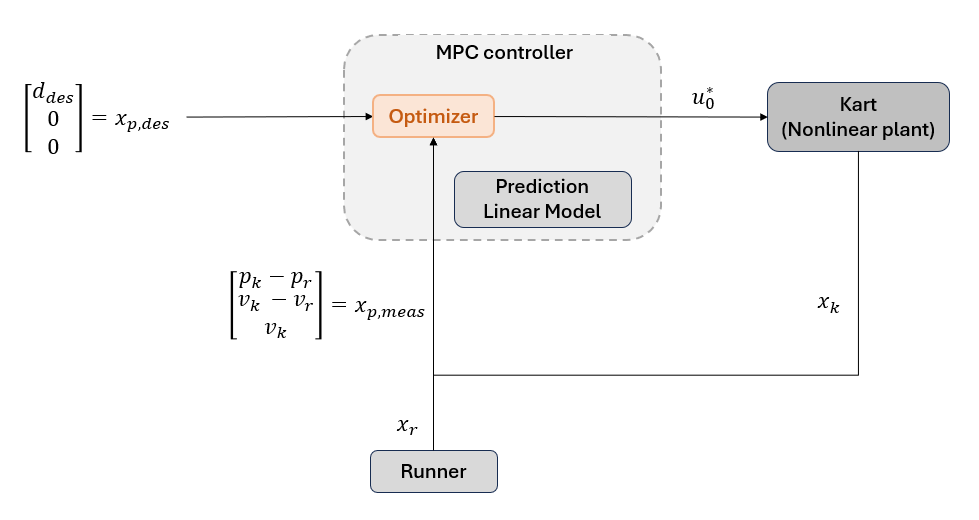
\includegraphics[width=1.0\textwidth]{MPC_sim_scheme.png}
	\caption{Model Predictive Control scheme}
	\label{image:MPC_sim_scheme}
\end{figure}

\begin{algorithm}
\begin{algorithmic}[1]
	\State Define desired prediction state $x_{p,\text{des}} = [d_{\text{des}}, 0, 0]^T$;
	\State Set initial runner position with a proper distance $\bar{d}$ from kart;
	\For{$t=0,1,2,..., t_{\text{end}}$}
		\State Take prediction state information $x_{p,t} = [\Delta p_t, \Delta v_t, v_{k,t}]^T$;
		\State Solve the constrained QP and get $\boldsymbol{u}^* = \{u_0, u_1, \cdots, u_N\}$; 
		\State Inject the first element of the optimal input sequence $u_0^*$ in the plant;
	\EndFor
\caption{MPC implementation}
\label{alg:MPC_sim_implementation}
\end{algorithmic}
\end{algorithm}

The overall MPC control scheme is shown in \ref{image:MPC_sim_scheme}.
It is easy to understand the semplification in the architecture achieved with the MPC, with respect to the LQR case shown in \ref{image:LQR_sim_scheme}.
 Algorithm \ref{alg:MPC_sim_implementation} describes the points of the MPC implementation.

\section{Offset-free MPC and disturbance observer design}
The MPC problem formulated in \ref{MPC_formulation} employs as prediction model a linear approximation of the kart dynamics (see \ref{Linear_system}), augmented with the runner model in \ref{Runner_model}.
However, this prediction model does not take into account the nonlinear term arising from the drag coefficient present in the identified kart dynamic equations in \ref{Plant_simplified}.
In particular the true nonlinear prediction model for the MPC should result in the following formulation:

\begin{equation}
\begin{aligned}
    \begin{bmatrix}
        \Delta p_{t+1}  \\
        \Delta v_{t+1} \\
        v_{k,t+1}
    \end{bmatrix}
    & =
    \begin{bmatrix}
        1 & dt & 0 \\
        0 & 1 & -dt\frac{C_f}{m} \\
        0 & 0 & 1-dt\frac{C_f}{m}
    \end{bmatrix}
    x_{p,t}
    +
    \begin{bmatrix}
        0 \\
        dt \frac{C_{m1}}{m} \\
        dt \frac{C_{m1}}{m}
    \end{bmatrix}
    u_t + 
    \begin{bmatrix}
    0 \\
    - dt a_{r,t} \\
    0
    \end{bmatrix} 
    -
    \begin{bmatrix}
    0 \\
    dt (\frac{C_{d}}{m} v_{k,t}^2) \\
    dt (\frac{C_{d}}{m} v_{k,t}^2)
    \end{bmatrix}
\end{aligned}
\label{Non-lin_prediction_model_MPC}
\end{equation}

where the last term includes the nonlinear, unmodelled drag effect, thus the $w$ in \ref{Plant_model_mismatch} representing the model-plant mismatch term within the offset-free MPC context.

\bigskip
Since MPC derives its solution based on the linear model in \ref{Prediction_model_MPC}, the performance of the controller are inherently tied to the magnitude of the unmodeled effects.
Consequently, optimal closed-loop performance may not be achievable using the nominal MPC formulation. 
Offset-free MPC is designed to handle this kind of situations where there are discrepancies between the nominal model used for prediction and the actual plant dynamics. 

\bigskip
Data-driven control strategies, on the contrary, do not require models and can implicitly manage uncertainties in processes. 
However, pure data-driven approaches, without any prior assumptions about process necessitate extensive data and typically employ slow exploratory techniques.
Recent control methodologies blend model-based techniques with data-driven approaches to overcome these limitations.
The reasoning used in this thesis to compensate for the model-plant mismatch term, combines a predictive control based on the linear prediction model, with a real-time estimation and compensation of the nonlinear term based on data from the system.
This control strategy dynamically estimates for this discrepancy using the prediction errors, thus the difference between the model's predictions and the actual system response.

Although offset-free MPC can mitigate model-plant mismatch, estimating real-time the disturbance from measurement errors, the observer introduces a delay. 
This delay has as a consequence the fact that the disturbance compensation may only be optimal at steady-state and not during transient when the disturbance varies.

\bigskip
Considering the problem statement presented in \ref{MPC:offset-free}, the affine term that takes into account the runner acceleration, has been added, similar to the nominal MPC case.

The prediction model in \ref{Augmented_model} is applied and it results to be:
\begin{equation}
\begin{aligned}
	x_{p,t+1} & =
    \begin{bmatrix}
        1 & dt & 0 \\
        0 & 1 & -dt\frac{C_f}{m} \\
        0 & 0 & 1-dt\frac{C_f}{m}
    \end{bmatrix}
    x_{p,t}
    +
    \begin{bmatrix}
        0 \\
        dt \frac{C_{m1}}{m} \\
        dt \frac{C_{m1}}{m}
    \end{bmatrix}
    u_t + 
    \begin{bmatrix}
    0 \\
    - dt a_{r,t} \\
    0
    \end{bmatrix} 
    -
    \begin{bmatrix}
    0 \\
    1 \\
    1
    \end{bmatrix}
	d_t \\
    d_{t+1} & = d_t
\end{aligned}
\label{Offset-free_prediction_model_MPC}
\end{equation}

Here $B_d = [0, 1, 1]^T$ signifies that the disturbance affects only in the second and third states, while the relative position prediction model remains unaffected by the mismatch with the plant.
For the purposes of this thesis the state is considered to be fully observable (i.e. $C = I_3$) and, as a consequence, the reference for the measured plant output is translated in reference for the plant states, thus $y_{\text{des}} = x_{p,\text{des}} = [d_{\text{des}}, 0, 0] ^T$.
Accordingly also $C_d = [0, 0, 0]^T$. 

\bigskip
The design of the observer plays a crucial role in enhancing the robustness of the proposed control scheme.
The observer gain matrices $L_x$ and $L_d$ are designed in such a way the poles of $(A_e + L C_e)$ are placed in $\lambda=[0.5, 0.51, 0.52, 0.53]^T$, ensuring the resultant matrix to be Hurwitz. 
The same weighting matrices $Q$ and $R$ utilized in the nominal MPC context are employed as weights.

\begin{figure}
	\centering
	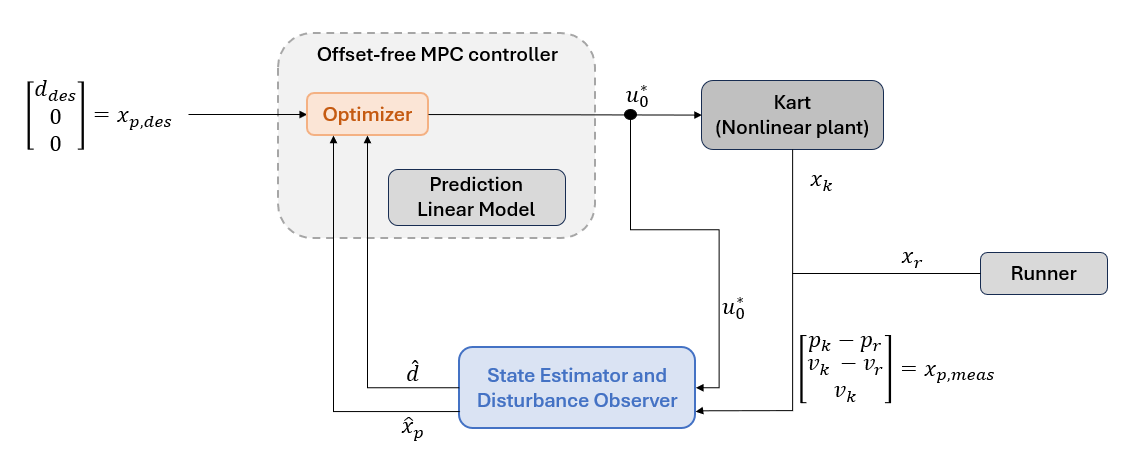
\includegraphics[width=1.0\textwidth]{MPC_of_scheme.png}
	\caption{Offset-free Model Predictive Control scheme with disturbance observer}
	\label{image:mpc_of_scheme}
\end{figure}

In image \ref{image:mpc_of_scheme} the block diagram of the proposed offset-free MPC with disturbance observer implementation is represented and algorithm \ref{alg:MPCOF_sim_implementation} describes the point of both estimation and control followed by the scheme.

\begin{algorithm}
\begin{algorithmic}[1]
	\State Define desired prediction state $x_{p,\text{des}} = [d_{\text{des}}, 0, 0]^T$;
	\State Set initial runner position with a proper distance $\bar{d}$ from kart;
	\State Initialize estimator $\hat{x}_{p,0} = [d_{\text{des}}, 0, 0]^T$ and $\hat{d}_0 = 0$;
	\For{$t=0,1,2,..., t_{\text{end}}$}
		\State Take state estimator and disturbance observer information $\hat{x}_{p,t}$ and $\hat{d}_t$;
		\State Solve the constrained QP and get $\boldsymbol{u}^* = \{u_0, u_1, \cdots, u_N\}$; 
		\State Inject the first element of the optimal input sequence $u_0^*$ in the plant;
		\State Update state estimator and disturbance observer 
	\EndFor
\caption{MPC Offset-free implementation}
\label{alg:MPCOF_sim_implementation}
\end{algorithmic}
\end{algorithm}



\chapter{Simulation results and Hardware-in-the-loop validation}
%\addcontentsline{toc}{chapter}{Simulations and Hardware results}
\markboth{}{RESULTS}
\label{chapter:Simulations_and_results}
The first purpose of this chapter is to present and analyze the results of Python simulations.

Later an overview of the hardware structure and sensors equipment of the system is provided together with the changes in the controllers formulations with respect to the simulation environment. 

Finally, some test developed on the real hardware are presented and their results are compared with the simulation framework.

\section{Simulation results}
This section presents the results obtained carrying out a Python simulation of the go-kart non linear dynamical model.
Two different velocity profiles for the runner are used as data and represented in figure (Plot solo profili velocità).
The three controllers: Linear Quadratic Regulator, Model Predictive Control and Offset-Free Model Predictive Control have been tested and their performances are evaluated and compared.

\begin{figure}[htbp]
    \centering
    \begin{subfigure}[t]{0.8\textwidth}
        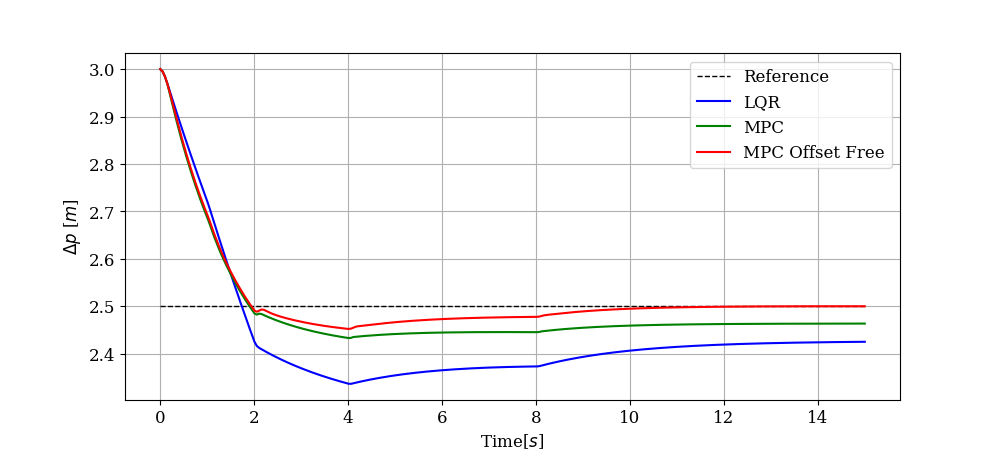
\includegraphics[width=\textwidth]{Test1/Deltap.png}
        \caption{Relative position}
        \label{fig:Deltap1}
    \end{subfigure}
    
    \begin{subfigure}[t]{0.8\textwidth}
        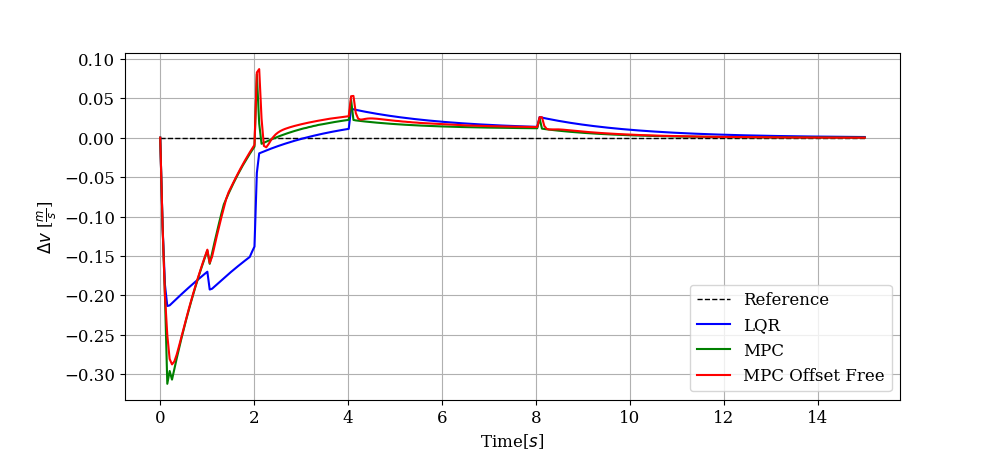
\includegraphics[width=\textwidth]{Test1/Deltav.png}
        \caption{Relative velocity}
        \label{fig:plot2}
    \end{subfigure}
    
    \begin{subfigure}[t]{0.8\textwidth}
        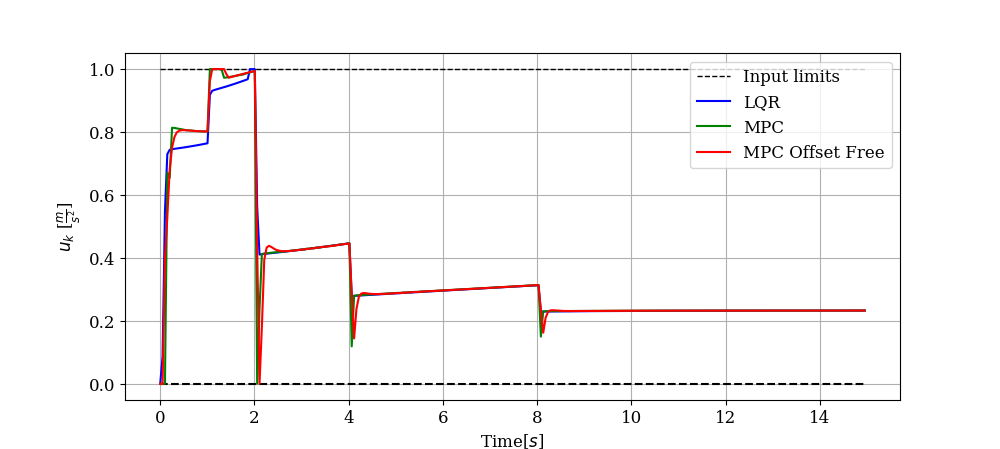
\includegraphics[width=\textwidth]{Test1/Input.png}
        \caption{T}
        \label{fig:plot3}
    \end{subfigure}
    \caption{Input}
    \label{fig:pannello}
\end{figure}

\begin{table}[htbp]
	\centering
	\caption{Comparison of controllers performances: First test}
	\label{tab:Test1}
	\begin{tabular}{c|c|c|c}
          & LQR & MPC & MPC Offset-free \\
	\hline
	\hline
	Mean($\Delta p$) & 0.1260 & 0.0681 &  0.0429 \\
	Mean($\Delta v$) & 0.0341 & 0.0265 & 0.0282 \\
	IAE on $\Delta p$ & 1.8759 & 1.0082 & 0.6304 \\
	IAE on $\Delta v$ & 0.5127 & 0.4009 & 0.4236 \\
	Min($\Delta p$) & 2.3366 & 2.4330 & 2.4523 \\
	Energy consumption & 0.3552 & 0.3548 & 0.3552 \\
	Steady state error [$cm$] & 0.0758 & 0.0365 & 0.0\\
	"Rise" time to  ${d}$ & 1.4 & 1.35 & 1.4 \\
	\hline
	\end{tabular}
\end{table}





\section{System structure and hardware description}
This part discuss the hardware components present in the system.



The system comprises a fully electric-powered go-kart with an attached airshield structure via a fixed joint. According to the CIK-FIA (International Karting Commission Federation International Automobile), a go-kart is a land vehicle with four non-aligned wheels in contact with the ground, two of which control steering while the others transmit power. Go-karts emerged after the post-war period of the 1950s, originally created by airmen as a pastime. Typically, go-kart chassis are constructed from steel pipes that provide both stiffness and flexibility to compensate for the lack of a suspension system and a differential.

\subsection*{Electric-powered go-kart}
The kart is a SinusIon purchased from the German company RiMO (originally Richter + Mohn). 

\bigskip
The battery on board is a lithium-iron-manganese-4-phosphate (LiFeMnPO4), used in order to reduce the battery pack weight.

\bigskip
For what regards the motor it's a Heinzmann PMS 100, with air-cooled cooling technology. 
This DC motor is a permanent magnet brush-less motor with a link voltage of 28V, a nominal speed of 6500 rpm and a rated torque of 3.82 Nm, representing respectively the rotational speed at which the motor is designed to operate optimally and the maximum rotational force that the motor can exert.
Talking about efficiency this motor is characterized with high-efficiency and energy-saving capabilities, the rated power output is 2.6kW. 
This parameter reflects the motor's ability to convert electrical energy into mechanical power.
The gearbox has a gear ratio of 1:7.

\bigskip
The computer on board is a AMD Ryzen MinisForum EliteMini X500 with an AMD Ryzen 7 5700G processor (8 cores with nominal frequency of 3.8GHz) coupled with a 16GB DDR4 RAM.

\subsection*{Airshield}

\begin{figure}
	\centering
	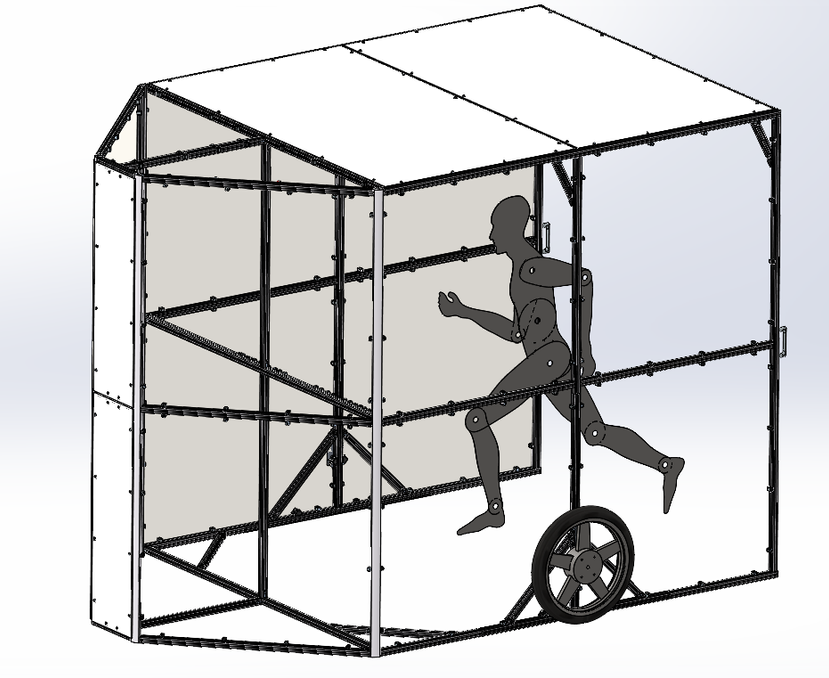
\includegraphics[width=0.5\textwidth]{Shield_structure.png}
\caption{Airshield structure}
\label{Shield_structure}
\end{figure}

The shield has the structure shown in \ref{Shield_structure}.
All the side and front panels are of plexiglass while the top part is an aluminium composite.

The dimensions are reported in table \ref{tab:Shield_dimensions}.

\begin{table}[h]
\centering
\begin{tabular}{|p{1.5cm}|p{1.5cm}|p{1.5cm}|}
\hline
Height & 2.15 m \\
\hline
Width & 1.86 m \\
\hline
Lenght & 2.95 m \\
\hline
\end{tabular}
\caption{Aishield dimensions}
\label{tab:Shield_dimensions}
\end{table}
The height can be adjusted inside a range of circa $13$ cm by simply moving a wheel bracket up or down, in order to better fit the height of the runner.

\section{Perception}
Autonomous vehicles sense and perceive the surrounding environment using measurements coming from sensors and then process the information in order to make informed decisions. 
This is the fundamental principle behind closed loop control that relies on measurements of controlled variables, provided by an appropriate sensor.
The perception systems used in autonomous vehicles are usually categorized in two groups:
\begin{itemize}
    \item Proprioceptive sensors (or internal state sensors) sensing the vehicle own state like wheel encoders or inertial measurement unit, location sensors like GPS, etc.
    \item Exteroceptive sensors (or external state sensors) gathering informations about the surrounding environment like cameras, LiDAR, RADARs, etc.
\end{itemize}
In this application the system is equipped with a LiDAR (Light Detection and Ranging), a camera, an inertial measurement unit and wheel encoders.

\subsection*{LiDAR}
LiDAR (Light Detected and Ranging) is a remote sensing technology that measures distances to objects and surfaces using laser pulses. 
The sensor consists of three main components: a laser emitter, a scanning mechanism, and a receiver.
The laser emitter sends out short pulses of laser light, which travel towards surrounding objects. 
When these pulses encounter an object they reflect off its surface and return to the LiDAR sensor.
The receiver than detects the reflected light and measures the time it takes for the pulses to return, allowing to calculate the distance of the object based on the speed of light.
Moreover, LiDAR rensors are capable of operating in various environmental conditions including darkness, rain, fow or low visibility, making them perfect for the application and highly reliable.

The LiDAR mounted on the airshield is a Velodyne VLP-16, a compact sensor that features 16 laser channels arranged in a circular configuration to have an important field of view.

The field of view (angular extension of a scene that is projected by the laser beam) is of 360$^\circ$ horizontal and 30$^\circ$ vertical.
The range of the laser is up to 100 m. 
Measures have an accuracy of +/- 3 cm and are acquired with a frequency of 20 Hz.

\subsection*{Camera}
Cameras provide rich information about the surrounding environment and can be used in a variety of ways.
On the airshield a ZED 2i Stereo Camera with polarized lens of 4mm is mounted.

The field of view is of 120$^\circ$ and the camera is able to sense ranges between 1.5 m and 35 m. 
The depth accuracy is smaller of the 2\% of the distance up to 10 m while it increases up to the 7\% for distances up to 30m distance.

The camera is equipped with a Stereolab ZED Box Xavier NX 8GB, an industrial compact and powerful mini PC used for computing and processing camera data.
It's powered with an NVIDIA Jetson embedded GPU.

At the moment LiDAR measurement are prefered with respect to camera ones thanks to the higher accuracy.
Camera remains responsible for the detection of the gesture to identify the moment in which the runner is able to start the performance. 

\subsection*{Wheel Encoder}
Rotary encoders are a type of sensor that measures the rotation of a mechanical shaft.
Two wheel encoders, one for each wheel, are integrated in the PMS 100 motor as speed sensors providing the motor rotational speed.
Then by knowing that the gear ratio is 1:7 and that the wheel diameter is $27.89$ cm the absolute go-kart speed can be evaluated as follows:

\begin{equation}
    v_{\text{kart}} = \frac{\pi \cdot d \cdot \text{avg rate}}{60 \cdot \text{gear ratio}}
\end{equation}
where avg rate is the average motor rate between left and right sides.



\subsection*{Inertial Measurement Unit}

\begin{figure}[h!]
	\centering
	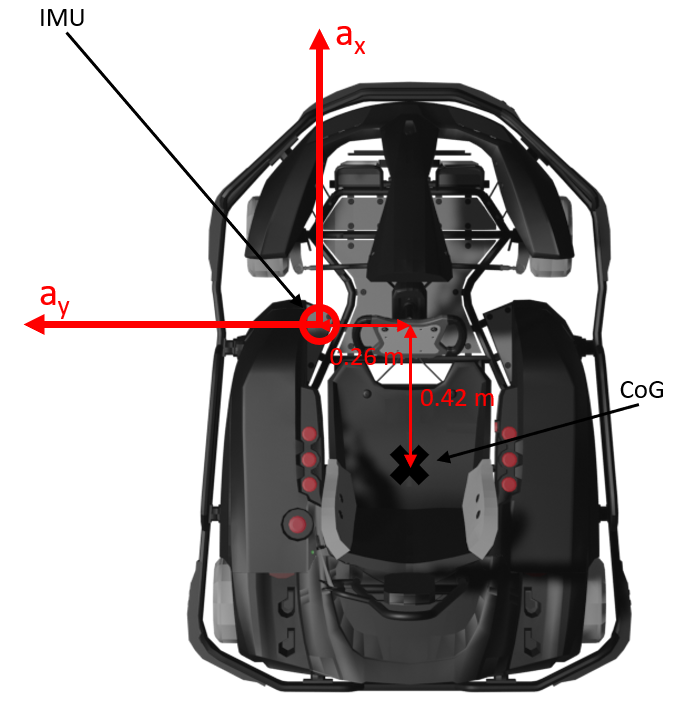
\includegraphics[width=0.3\textwidth]{IMU.png}
\caption{IMU position on the go-kart}
\label{IMU_pose}
\end{figure}

Typically an IMU or Inertial Measurement Unit consists of a combination of accelerometers and a gyroscopes, and sometimes also magnetometers in order to measure the orientation, velocity and acceleration of an object.
Thanks to the combination of accelerometers and gyroscopes the IMU is able to sense the object orientation or angular motion and acceleration with respect to some predefined axes.
The IMU used in the go-kart is the IRIMU-V2 from Izze-Racing that outputs data at 200Hz via CAN protocol and has an accuracy of less than 1\% of full scale for the acceleration and less than 1.5\% for the angular acceleration.
The position with respect to the go-kart centre of gravity is showed in \ref{IMU_pose}.


\subsection{Controller design changes for hardware integration}
In the context of the hardware control implementation the available informations are the one coming from sensors and we cannot rely on a full state knowledge for both runner and kart as hypotized in Chapter 2.
For this reason we have to take into account the sensor present in the system and the measurement provided by them to control the system properly. 

\subsubsection*{LQR}
Differently from the simulation context, where all the state variables both for runner and kart have been considered to be fully known, in the hardware-in-the-loop context, absolute position of both kart and runner, as well as the runner absolute velocity, result to be unknown.

\begin{figure}
	\centering
	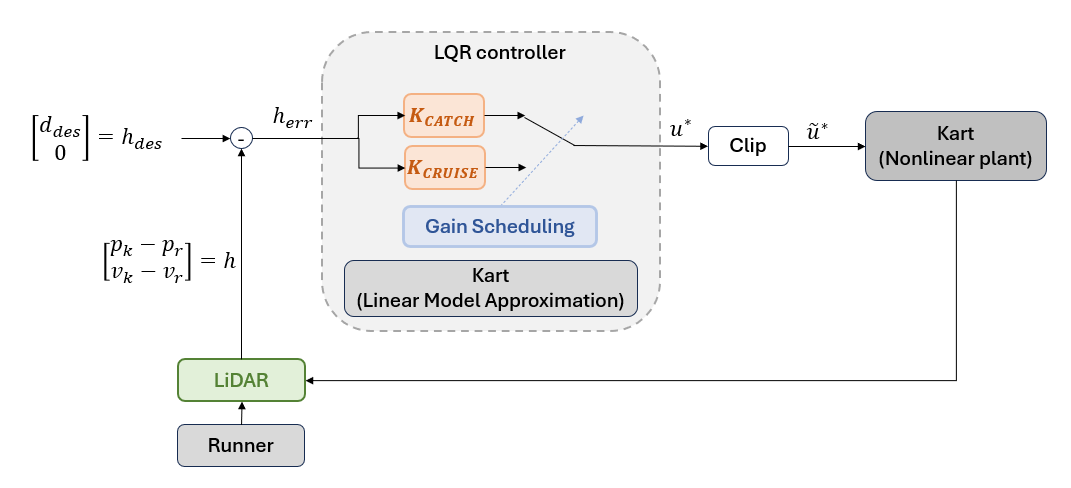
\includegraphics[width=1.0\textwidth]{LQR_hard_scheme.png}
	\caption{Linear Quadratic Regulator scheme with sensors}
	\label{image:LQR_hard_scheme}
\end{figure}

The LiDAR, as a range sensor, provides directly the measurement of the relative distance between runner and kart $\Delta p$, while the relative velocity can be estimated via finite differences:

\begin{equation}
	\Delta v_t = \frac{\Delta p_t - \Delta p_{t-1}} {dt}
\end{equation}
where $\Delta p_t := p_{k,t} - p_{r,t}$ and $\Delta v_t := v_{k,t} - v_ {r,t}$, and $dt$ is the sampling time.

The third component of the prediction state, the kart absolute velocity, is obtained from the wheel encoders.

\begin{algorithm}
\begin{algorithmic}[1]
	\State catched = false;
	\State Set initial runner position with a proper distance $\bar{d}$ from kart;
	\State Define desired system behaviour  $h_{\text{des}} = [d_{\text{des}}, 0]^T$;
	\For{$t=0,1,2,...$};
		\State Take LiDAR information $h_t = [\Delta p_t, \Delta v_t]^T$;
		\State Take absolute kart velocity $v_{k,t}$ from wheel encoders;
		\State Evaluate absolute runner velocity $v_{r,t} = v_{k,t} - \Delta v_t $;
		\If{$v_{k,t} \geq 0.8 \, v_{r,t}$ \textbf{and} catched = false}
			\State catched = true;
		\EndIf
		\If{catched = false}
			\State $u^* = - K_{\text{catch}} (h_t - h_{\text{des}}) $;
		\Else 
			\State $u^* = - K_{\text{reg}} (h_t - h_{\text{des}}) $;
		\EndIf
		\State Clip input according to limit saturation limits $\tilde{u}^* = \text{sat}_{[a_{\min}, a_{\max}]} (u^*)$;
		\State Inject $\tilde{u}^*$ in the plant;
	\EndFor
\caption{LQR implementation on hardware system}
\label{alg:LQR_hard_implementation}
\end{algorithmic}
\end{algorithm}

\bigskip
The closed loop control law in \ref{Closed-loop_control_law} can be modified as follows to directly use the measurments provided by the LiDAR to evaluate the feedback error and compute the current control action:
\begin{equation}
    u_t^* = K (h_t - h_{\text{des}})
\label{Closed-loop_control_law_sensors}
\end{equation}

where 
\begin{equation}
    h_t =
    \begin{bmatrix}
        \Delta p_t  \\
        \Delta v_t
    \end{bmatrix}
	=
    \begin{bmatrix}
        p_{k,t} - p_{r,t} \\
        v_{k,t} - v_{r,t}
    \end{bmatrix},
    \quad
    h_{\text{des}} =
    \begin{bmatrix}
        d_{\text{des}} \\
        0
    \end{bmatrix}.
\end{equation}



\subsection*{MPC}
\begin{figure}
	\centering
	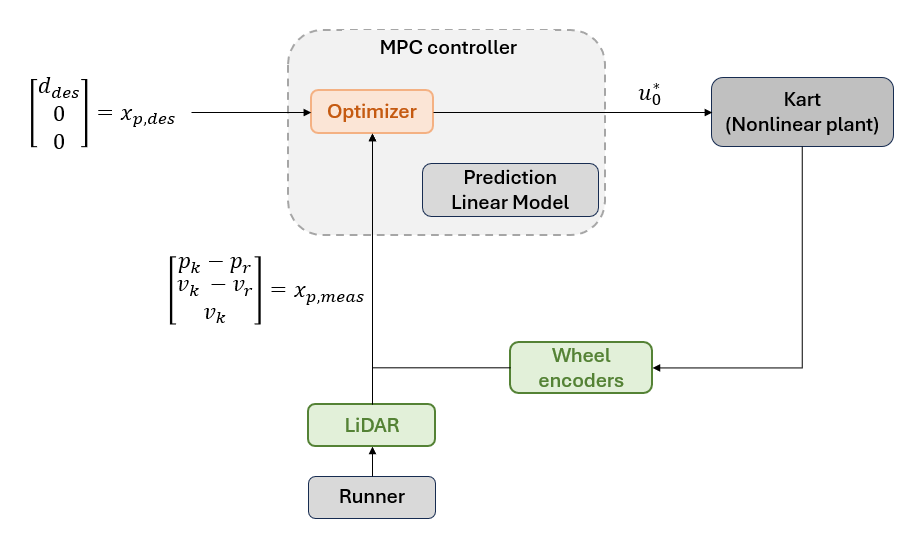
\includegraphics[width=1.0\textwidth]{MPC_hard_scheme.png}
	\caption{Model Predictive Control scheme with sensors}
	\label{image:MPC_hard_scheme}
\end{figure}

The overall implementation of the LQR in the context of the real system in described by algorithm \ref{alg:LQR_hard_implementation}, while the control architecture using the sensors for taking the measurements is shown in figure \ref{image:MPC_hard_scheme}.

It has to be noticed that the actual absolute runner acceleration is estimated. 
First of all the relative acceleration between kart and runner $\Delta a$ is estimated, as well as the kart absoluted acceleration $a_k$.
The absolute runner acceleration used is equal to $a_r = a_k - \Delta a$.
For this purpose a Kalman filter has been used.

Tutto il discorso sul noise



	  
	

%%%%%%%%%% APPENDIX %%%%%%%%%%%%%%%%%%%

%\appendix
%\chapter{Appendix title}


%%%%%%%%%% BIBLIOGRAPHY %%%%%%%%%%%%%%

\printbibliography


\addcontentsline{toc}{chapter}{Bibliography}
%%%%%%%%%%%%%%%%%%%%%%%%%%%%%%%%%%%%%%

\end{document}